\section{Hardware Side - Delivery Architecture} 

YouTube was released in 2005 and had an immediate success, resulting in a stunning growth ever since. This growth led to changes in the infrastructure, so that is today more flexible and scalable. In late 2007 Google acquired YouTube and the delivery architecture that initially used third party content distribution network services is now fully operated and managed by Google.
\\
\\
Describing a system like YouTube that constantly evolves is not easy, but a lot of the underlying design principles will most likely stay the same for some time.

\subsection{Steps of downloading a YouTube Video}

Watching a video on YouTube includes downloading the video (or parts of the video) to a client. This downloading process involves different sets of servers, which are necessary for load balancing. The high level steps of accessing a YouTube video are shown in Figure~\ref{fig:video_retrieval}:

\begin{figure}[htbp]
  \begin{center}
    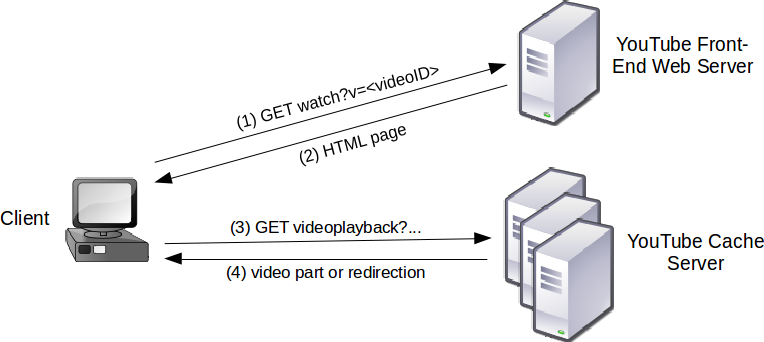
\includegraphics[width=\textwidth]{pictures/video_retrieval.png}
    \caption{High level sequence of steps to retrieve a YouTube video}
    \label{fig:video_retrieval}
  \end{center}
\end{figure}

\begin{enumerate}
  \item The client requests a specific video on the YouTube web page via http://www.youtube.com/watch?v=<videoID>. YouTube has multiple front-end servers for client requests, whereby one server will be responsible for a single request (without considering server crashes).
  
  \item The client downloads the corresponding HTML page. Depending on the video and the profile configuration, the actual video is either embedded through a Adobe Flash Player plugin or a HTML5 video container\footnote{YouTube currently tries to use the HTML5 player always when possible\cite{misc:youtube_html5}}. The relevant container takes further care of the download and the playback of the video. The name of the cache server that will provide the video is among the parameters provided for the plugin or the HTML5 container \cite{inpr:server_selection}.
  
  \item The respective cache server will be queried for the first video part via \seqsplit{https://<hostname>.googlevideo.com/videoplayback?<request-parameter>}. 

  \item If the cache server has the video and is not overloaded, the server will send the first part of the video ot the client. The client on the other hand will send requests for further video parts, if he keeps watching the respective video part. \\
\\
If the cache server does not have the video or is overloaded, the server will send a redirect message (HTTP 302) to the client indicating another cache server. The request process continues at step 3 again. Thus it is possible, that multiple cache servers are included in the request process.

\end{enumerate}

\subsection{Cache Server Infrastructure}

The cache servers themselves

\subsection{Cache Server Selection}
\label{subs:cache_server_selection}
